\section{Final testing and conclusions}\label{sec:conclusions}

Once we refined our model at the best could, we evaluated it against never seen data, by comparing the values predicted by the model, when the testing set is provided as input, against the true values of the annotations in the testing set. As already mentioned in section~\ref{sec:cross-validation}, once the final testing was done, we avoided going back to the model and make further tweaks, as this would have led to over-fitting.

\begin{table}
	\centering
	\subcaptionbox{MSEs}{
		\begin{tabular}{lcccc}
			\toprule
			& valence mean & valence std & arousal mean & arousal std \\
			\midrule
			Ridge & 0.53 & 1.09 & 0.54 & 1.18 \\
			$\nu$-SVM & 0.58 & 1.00 & 0.49 & 1.09 \\
			K-neighbors & 0.62 & 1.00 & 0.61 & 1.08 \\
			\bottomrule
		\end{tabular}
	}
	\subcaptionbox{$R^2$-scores}{
		\begin{tabular}{lcccc}
			\toprule
			& valence mean & valence std & arousal mean & arousal std \\
			\midrule
			Ridge & 0.45 \inc{-0.01} & -0.08 \inc{-0.04} & 0.45 \inc{+0.04} & -0.09 \inc{-0.01} \\
			$\nu$-SVM & 0.40 \inc{+0.00} & 0.01 \inc{+0.00} & 0.50 \inc{+0.02} & 0.00 \inc{-0.01} \\
			K-neighbors & 0.35 \inc{-0.05} & 0.01 \inc{+0.07} & 0.39 \inc{-0.01} & 0.00 \inc{+0.07} \\
			\bottomrule
		\end{tabular}
	}
	\caption{Final evaluation metrics}
	\label{table:eval-metrics}
\end{table}

For the final test we used the metrics of MSE and $R^2$-score (see section~\ref{sec:metrics}) and obtained the values reported in table~\ref{table:eval-metrics}, providing the differences in respect to table ~\ref{table:cross-scores}. It can be noticed that such differences fall between the confidence intervals provided by the cross-validation, therefore we can conclude that we still obtained a robust, albeit inaccurate, model, providing similar results in new unknown scenarios.

\begin{figure}
	\centering
	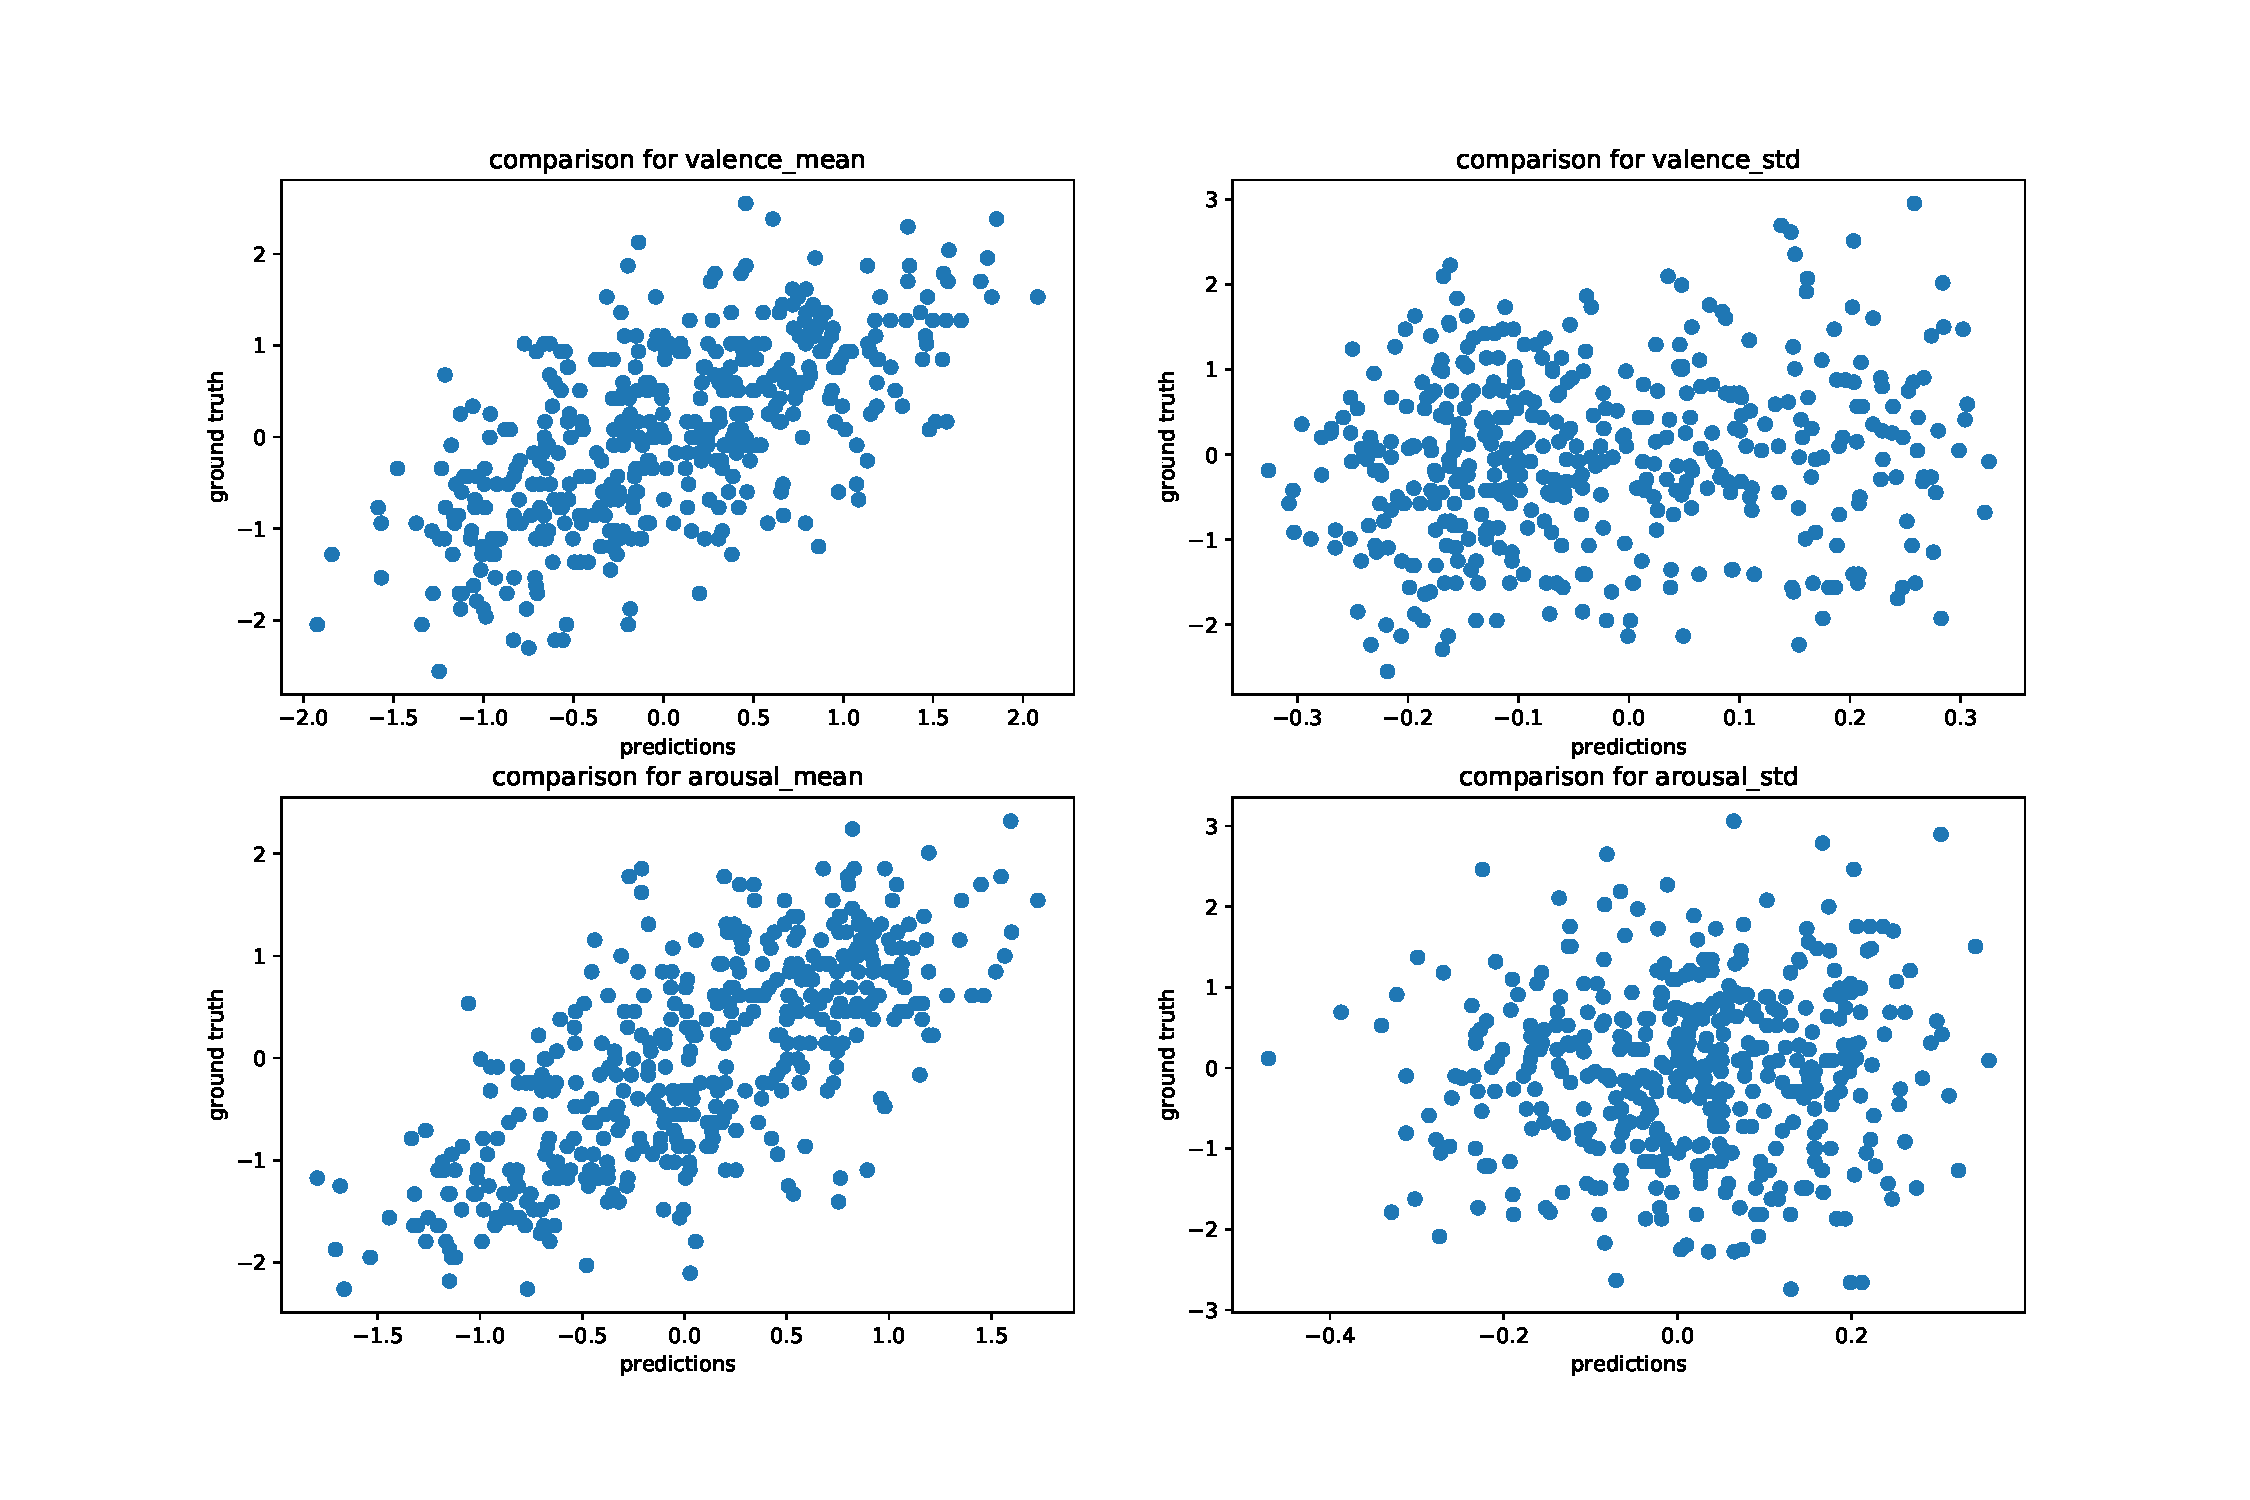
\includegraphics[width=\linewidth]{assets/predictions-scatter.pdf}
	\caption{predictions vs. ground-truth scatter for SVM regression}
	\label{fig:eval-scatter}
\end{figure}

We also extracted scatter plots comparing the predictions of each regressor against the true values of the testing set. In  figure~\ref{fig:eval-scatter} is depicted the case of $\nu$-SVM, which turned out to be the best model fitting the data. In the best case scenario, these scatters should draw a 45° line. In our case, the scattering of ``valence std'' and ``arousal std'' clearly outline the bad $R^2$-scores obtained for these annotations.

In our assignment, it was requested to use the static annotations and elaborate a regression model over static features. A possible way to develop and improve the accuracy of the obtained models could be to adopt a dynamic approach, in which values related to temporal windows are considered instead.
